\section{Manual de usuario}

\subsection{Introducción}
Este manual ha sido escrito con la finalidad de explicar clara y
sencillamente las funcionalidades disponibles en la aplicación. Para ello se
hará uso de capturas de pantalla de la propia aplicación acompañadas siempre
de un breve texto descriptivo.

\subsection{Registro}
\begin{figure}[!h]
    \centering
    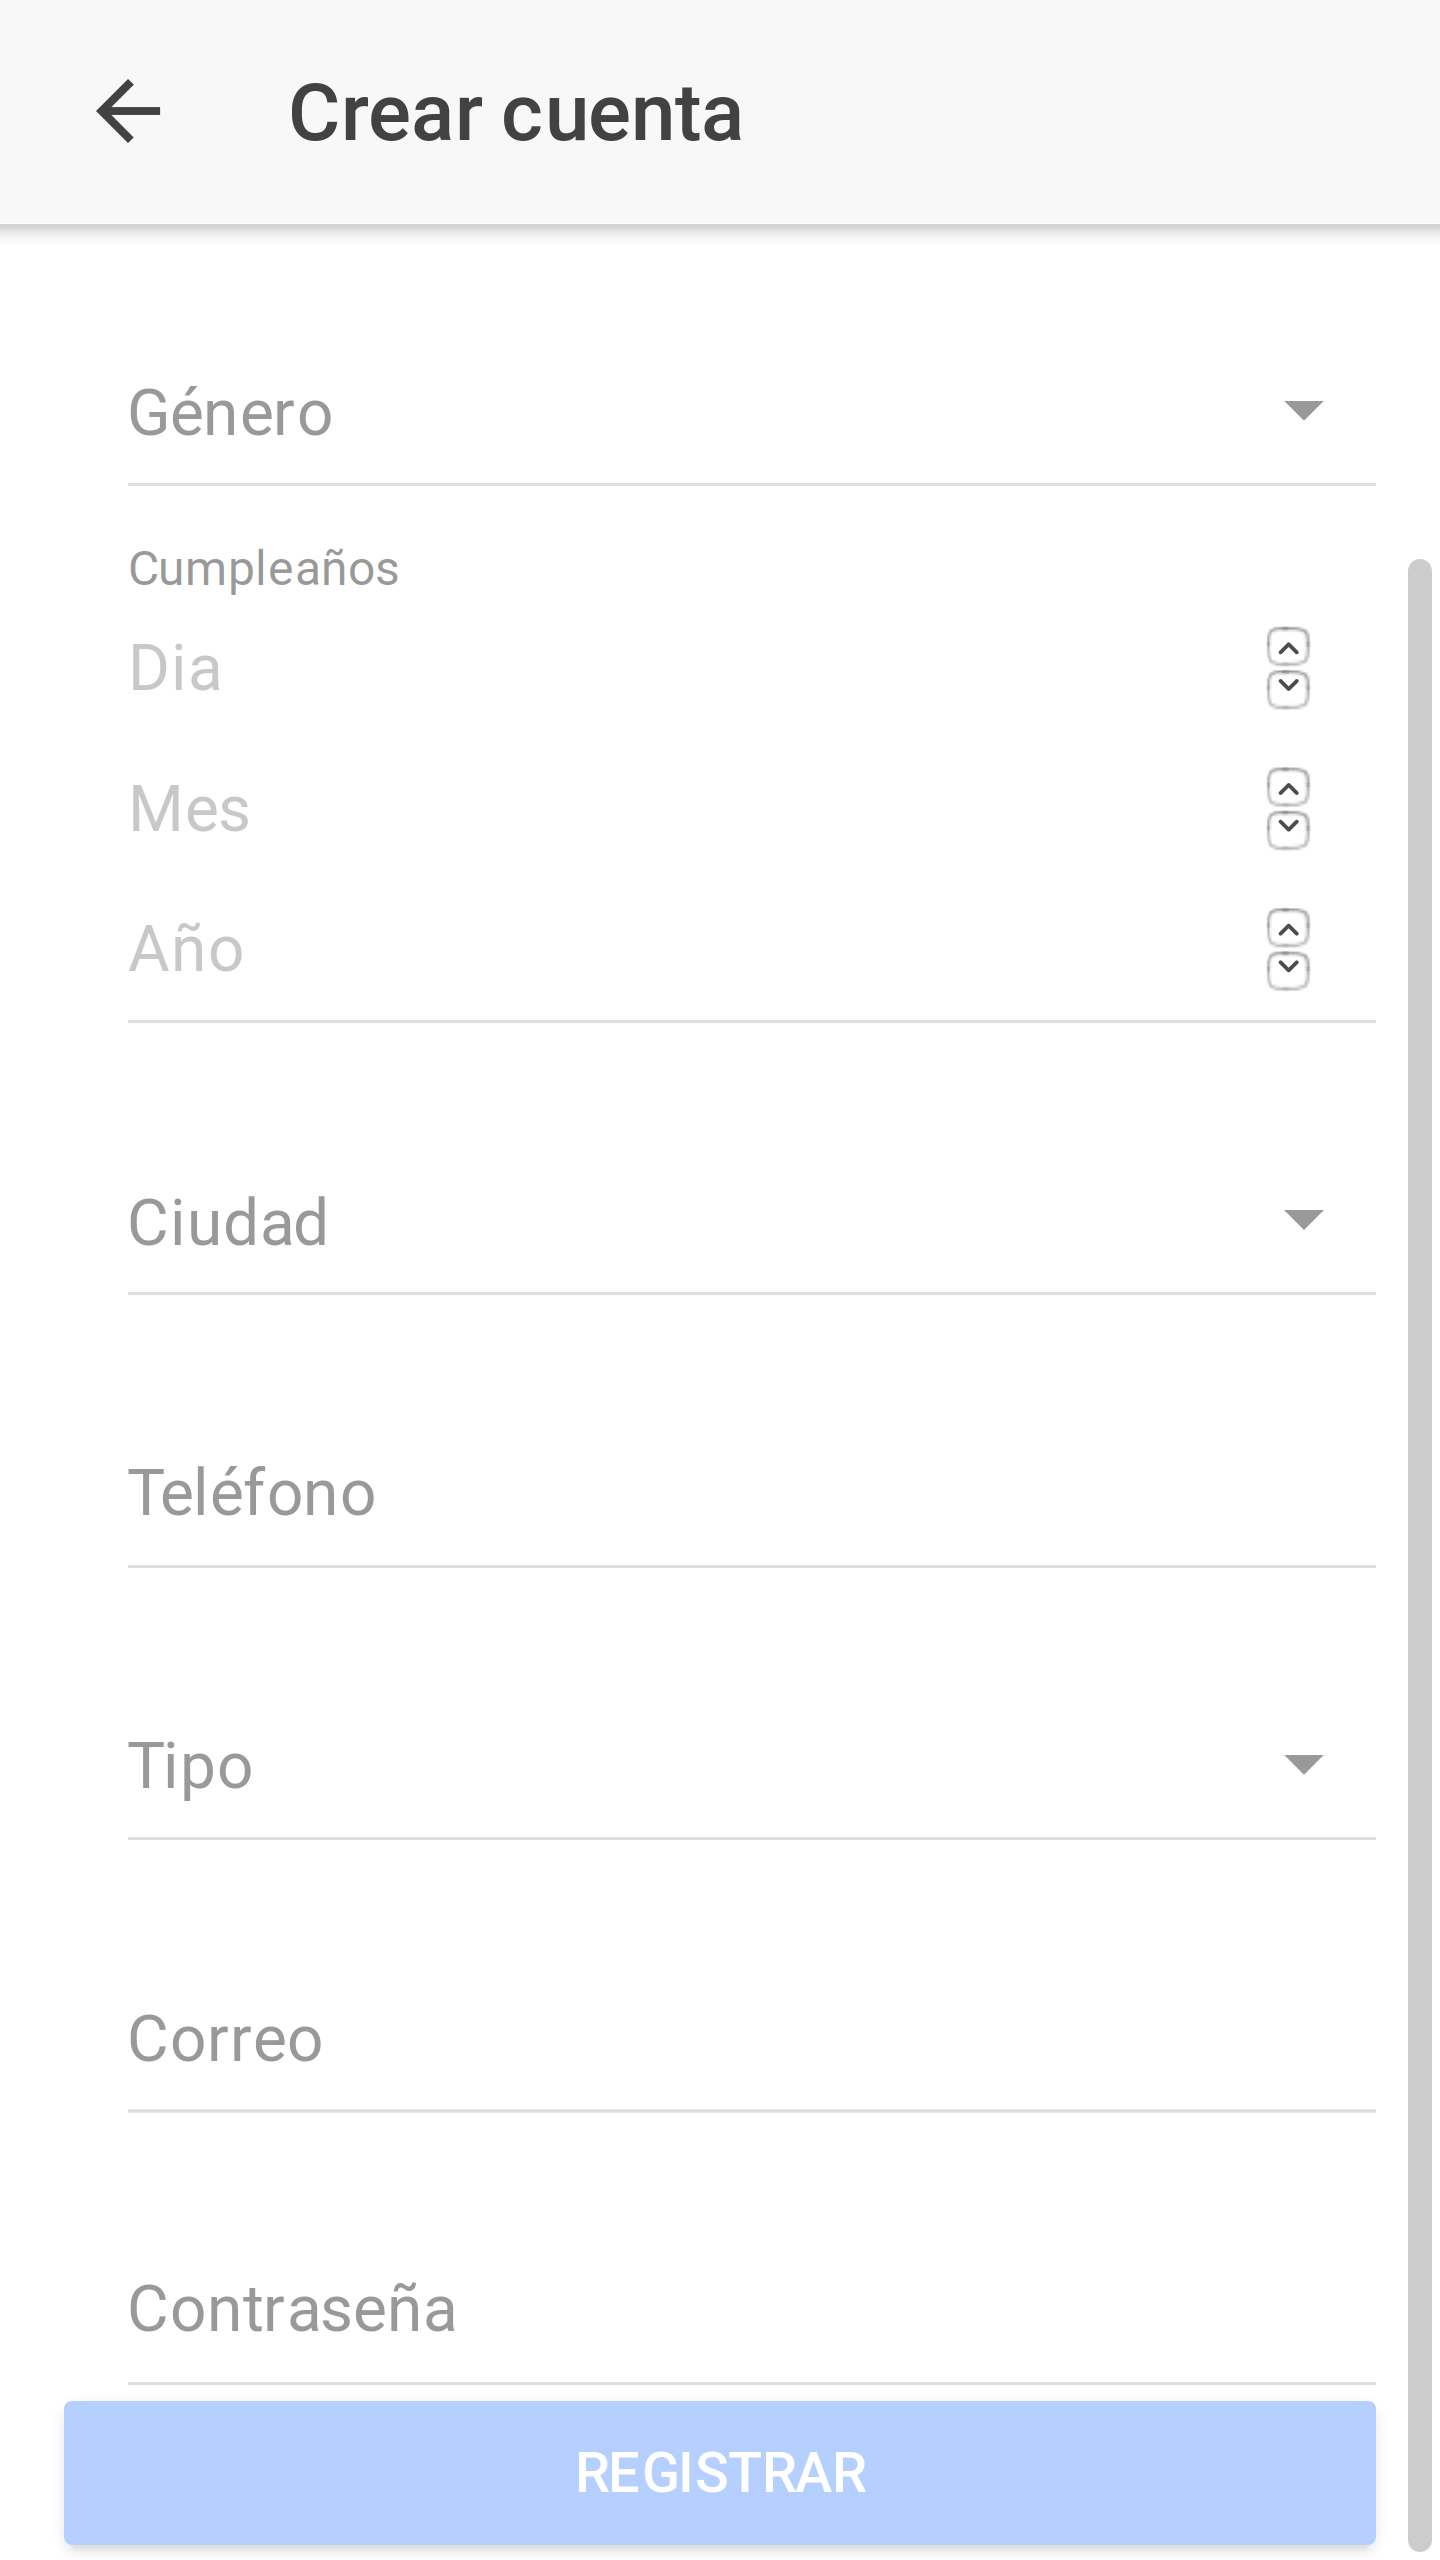
\includegraphics[width=0.4\textwidth]{images/screenshots/Registro.png}
    \caption{Formulario de registro}
    \label{formulario-registro}
\end{figure}

Antes de hacer uso de las funcionalidades de las que dispone la aplicación
los usuarios han de darse de alta. Para ello existe una ventana en la
aplicación en la que completar los datos del registro, como se puede ver en
la figura \ref{formulario-registro}.
\clearpage

\subsection{Inicio de sesión}
\begin{figure}[!h]
    \centering
    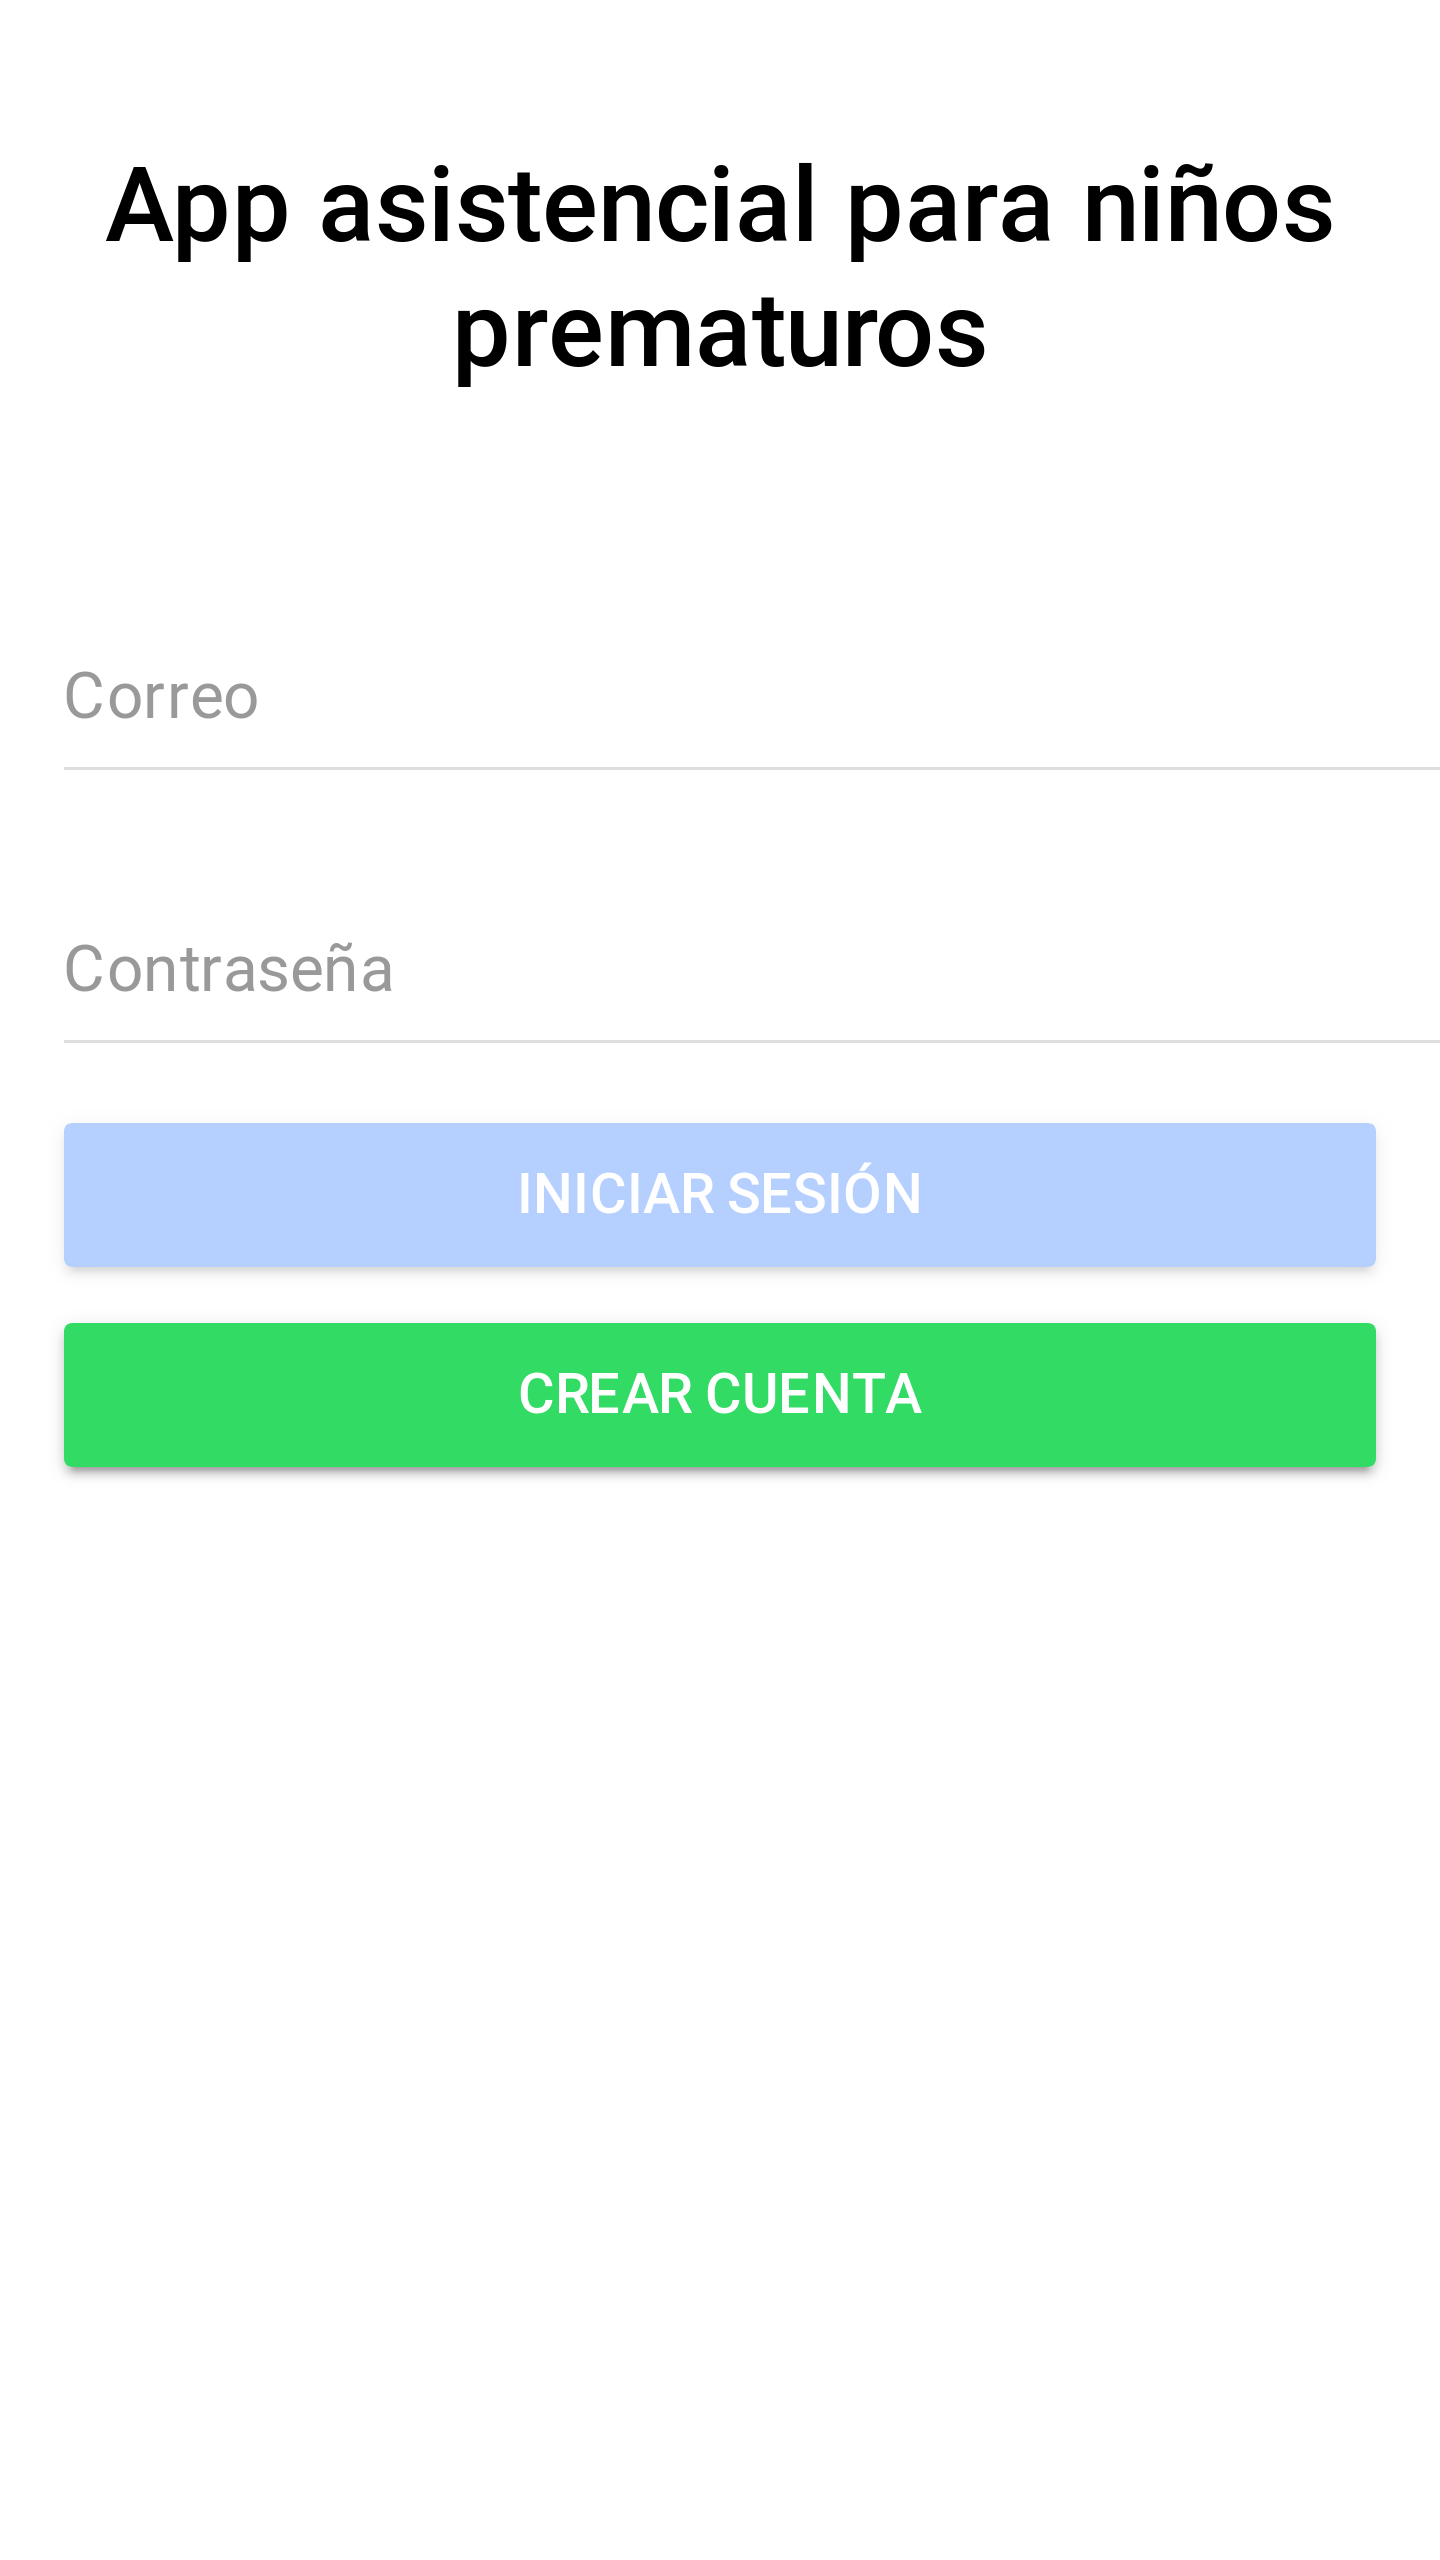
\includegraphics[width=0.5\textwidth]{images/screenshots/Pantalla-inicial.png}
    \caption{Formulario inicio de sesión}
    \label{formulario-inicio-sesion}
\end{figure}

Para poder acceder a la aplicación el usuario tiene que haber iniciado su
sesión previamente. Es por ello que la primera ventana que se muestra, en caso
de no estar en una sesión activa, es el formulario de inicio de sesión que se
puede ver en la figura \ref{formulario-inicio-sesion}.
\clearpage

\subsection{Barra de navegación}
\begin{figure}[!h]
    \centering
    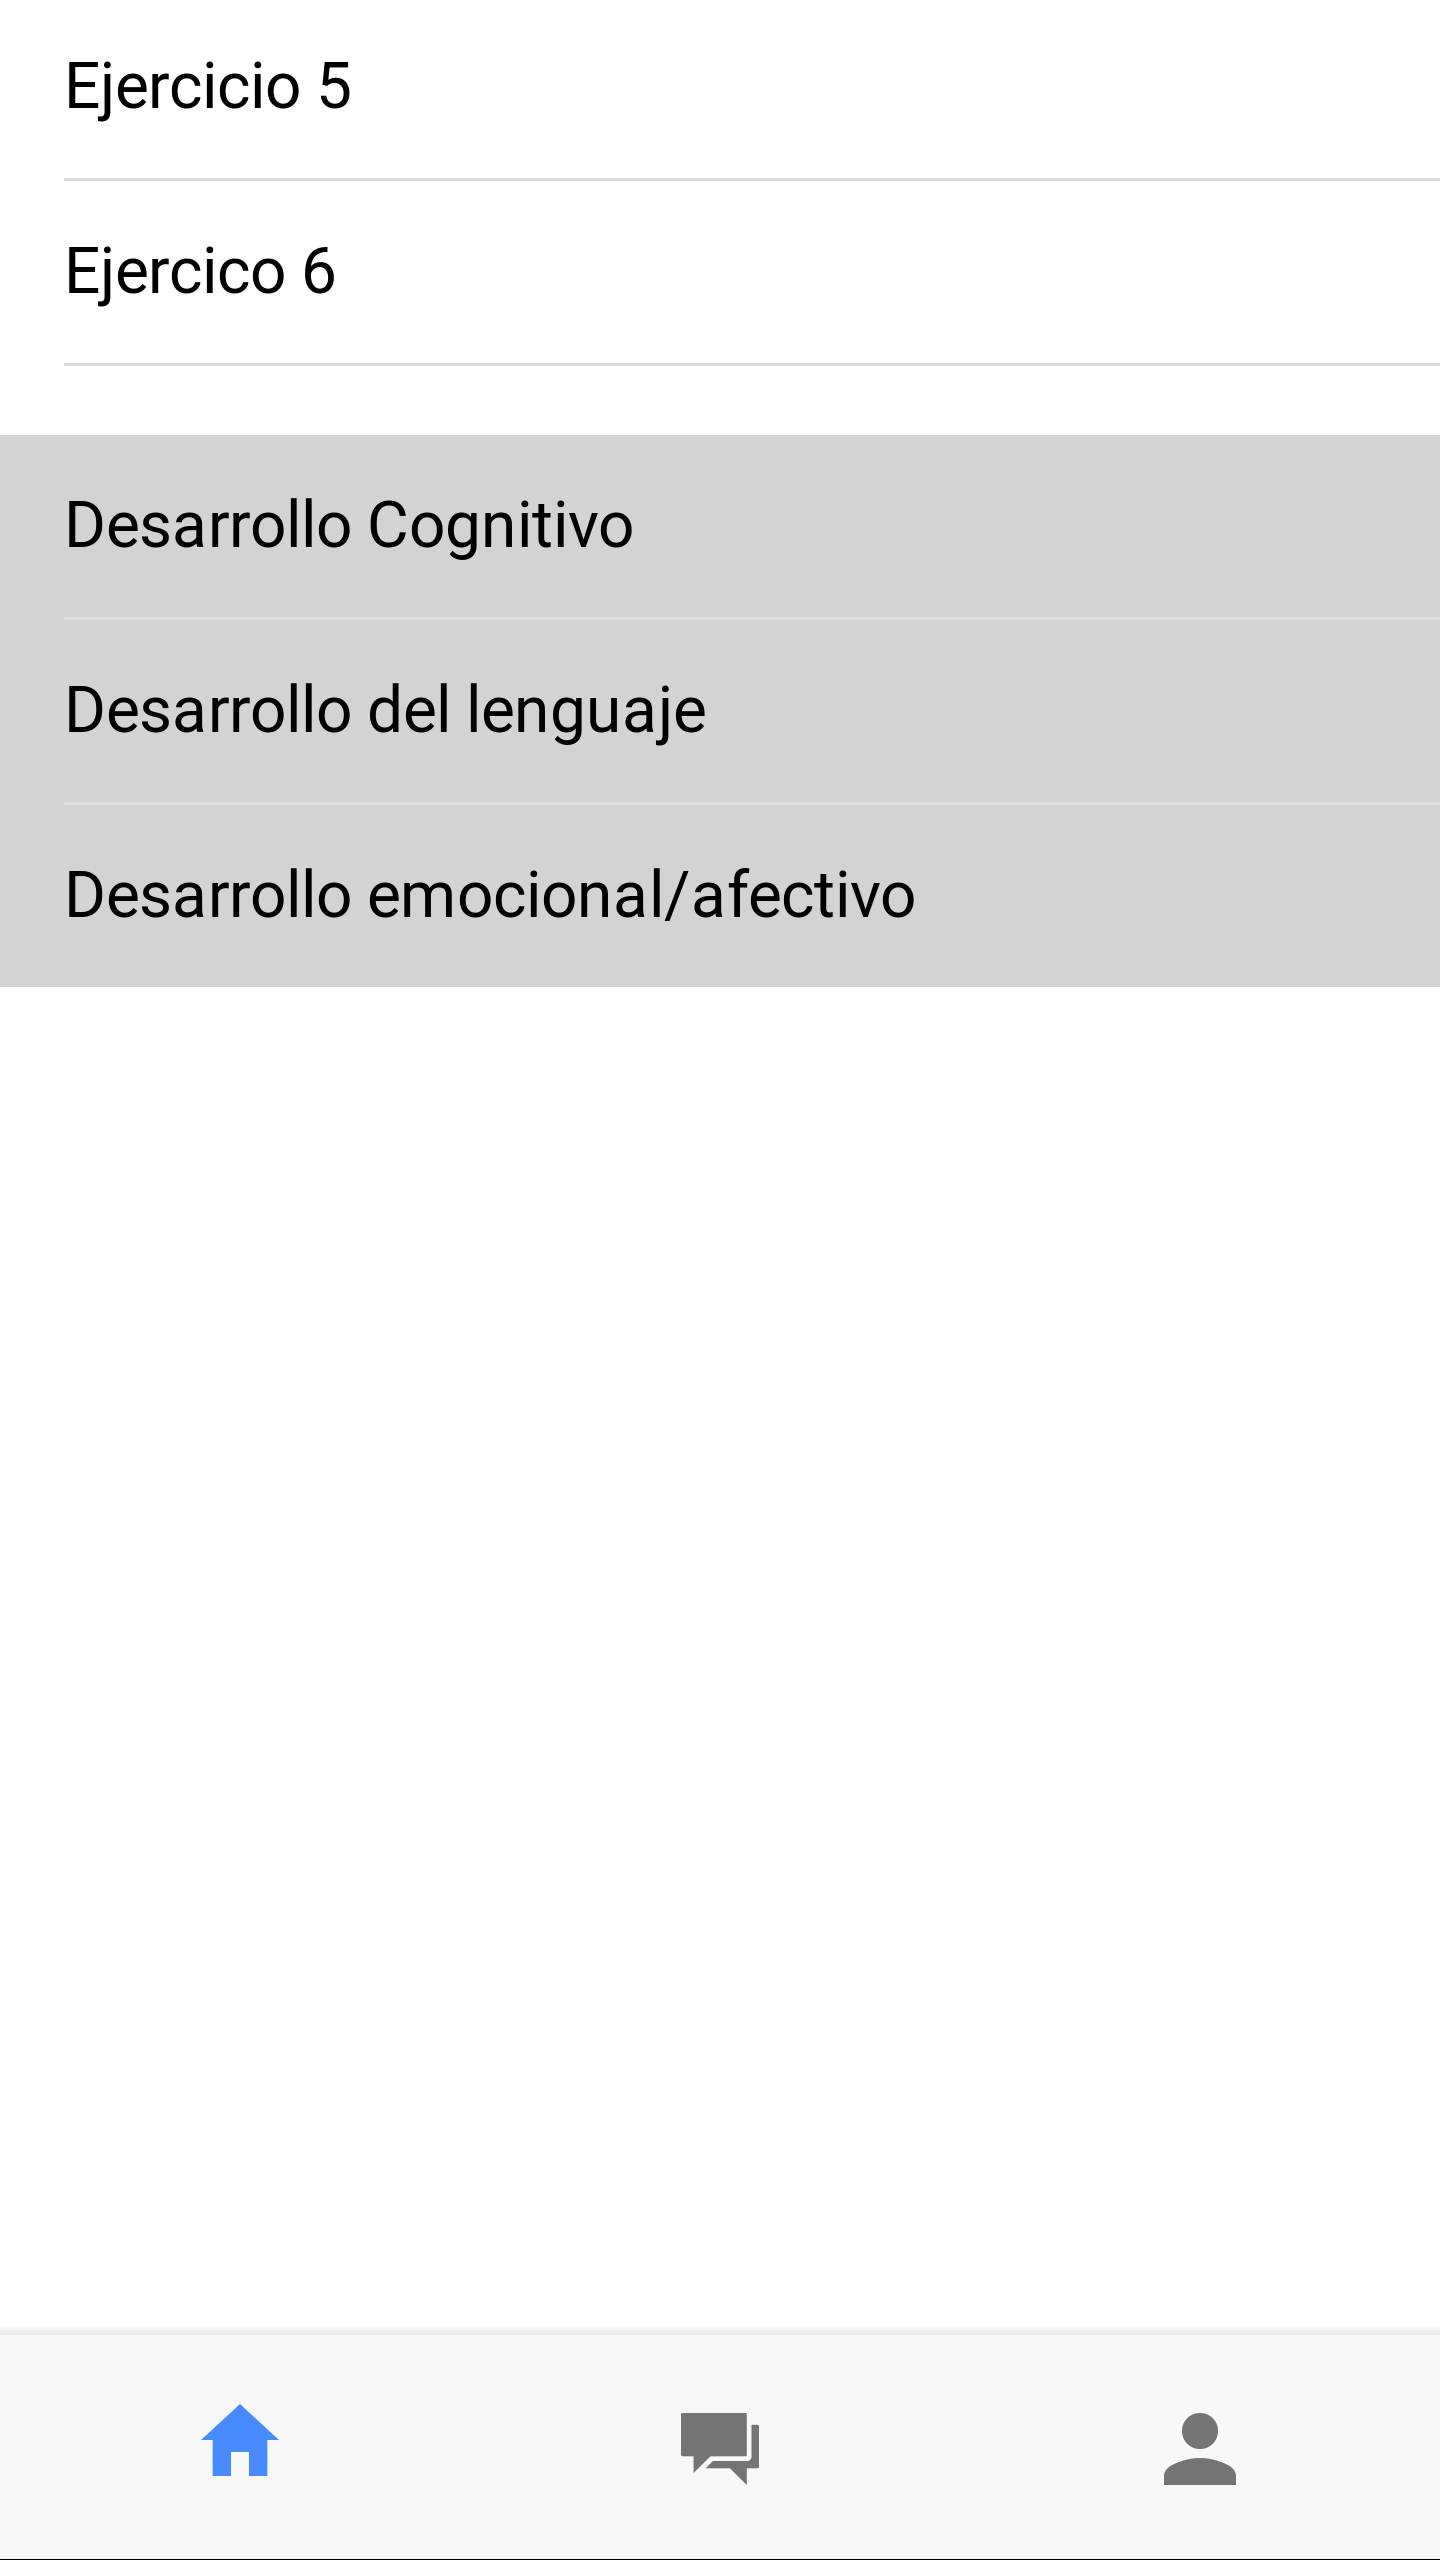
\includegraphics[width=0.5\textwidth]{images/screenshots/Paciente-ventana-principal.png}
    \caption{Pantalla principal, paciente}
    \label{pantalla-principal-paciente}
\end{figure}

En la figura \ref{pantalla-principal-paciente} se puede ver en la parte
inferior una barra de navegación. Esta barra está disponible en todas las
vistas de la aplicación. Con ella el usuario podrá navegar entre las
distintas opciones disponibles. Estas están indicadas con iconos
representativos de las mismas. Como son: página principal (\textit{home}),
chats y mi perfil, respectivamente. En el caso de los doctores, estos tienen
una pestaña adicional con el icono de una lupa donde podrán buscar entre los
pacietes registrados en la aplicación.
\clearpage

\subsection{Perfil de usuario}
\begin{figure}[!h]
    \centering
    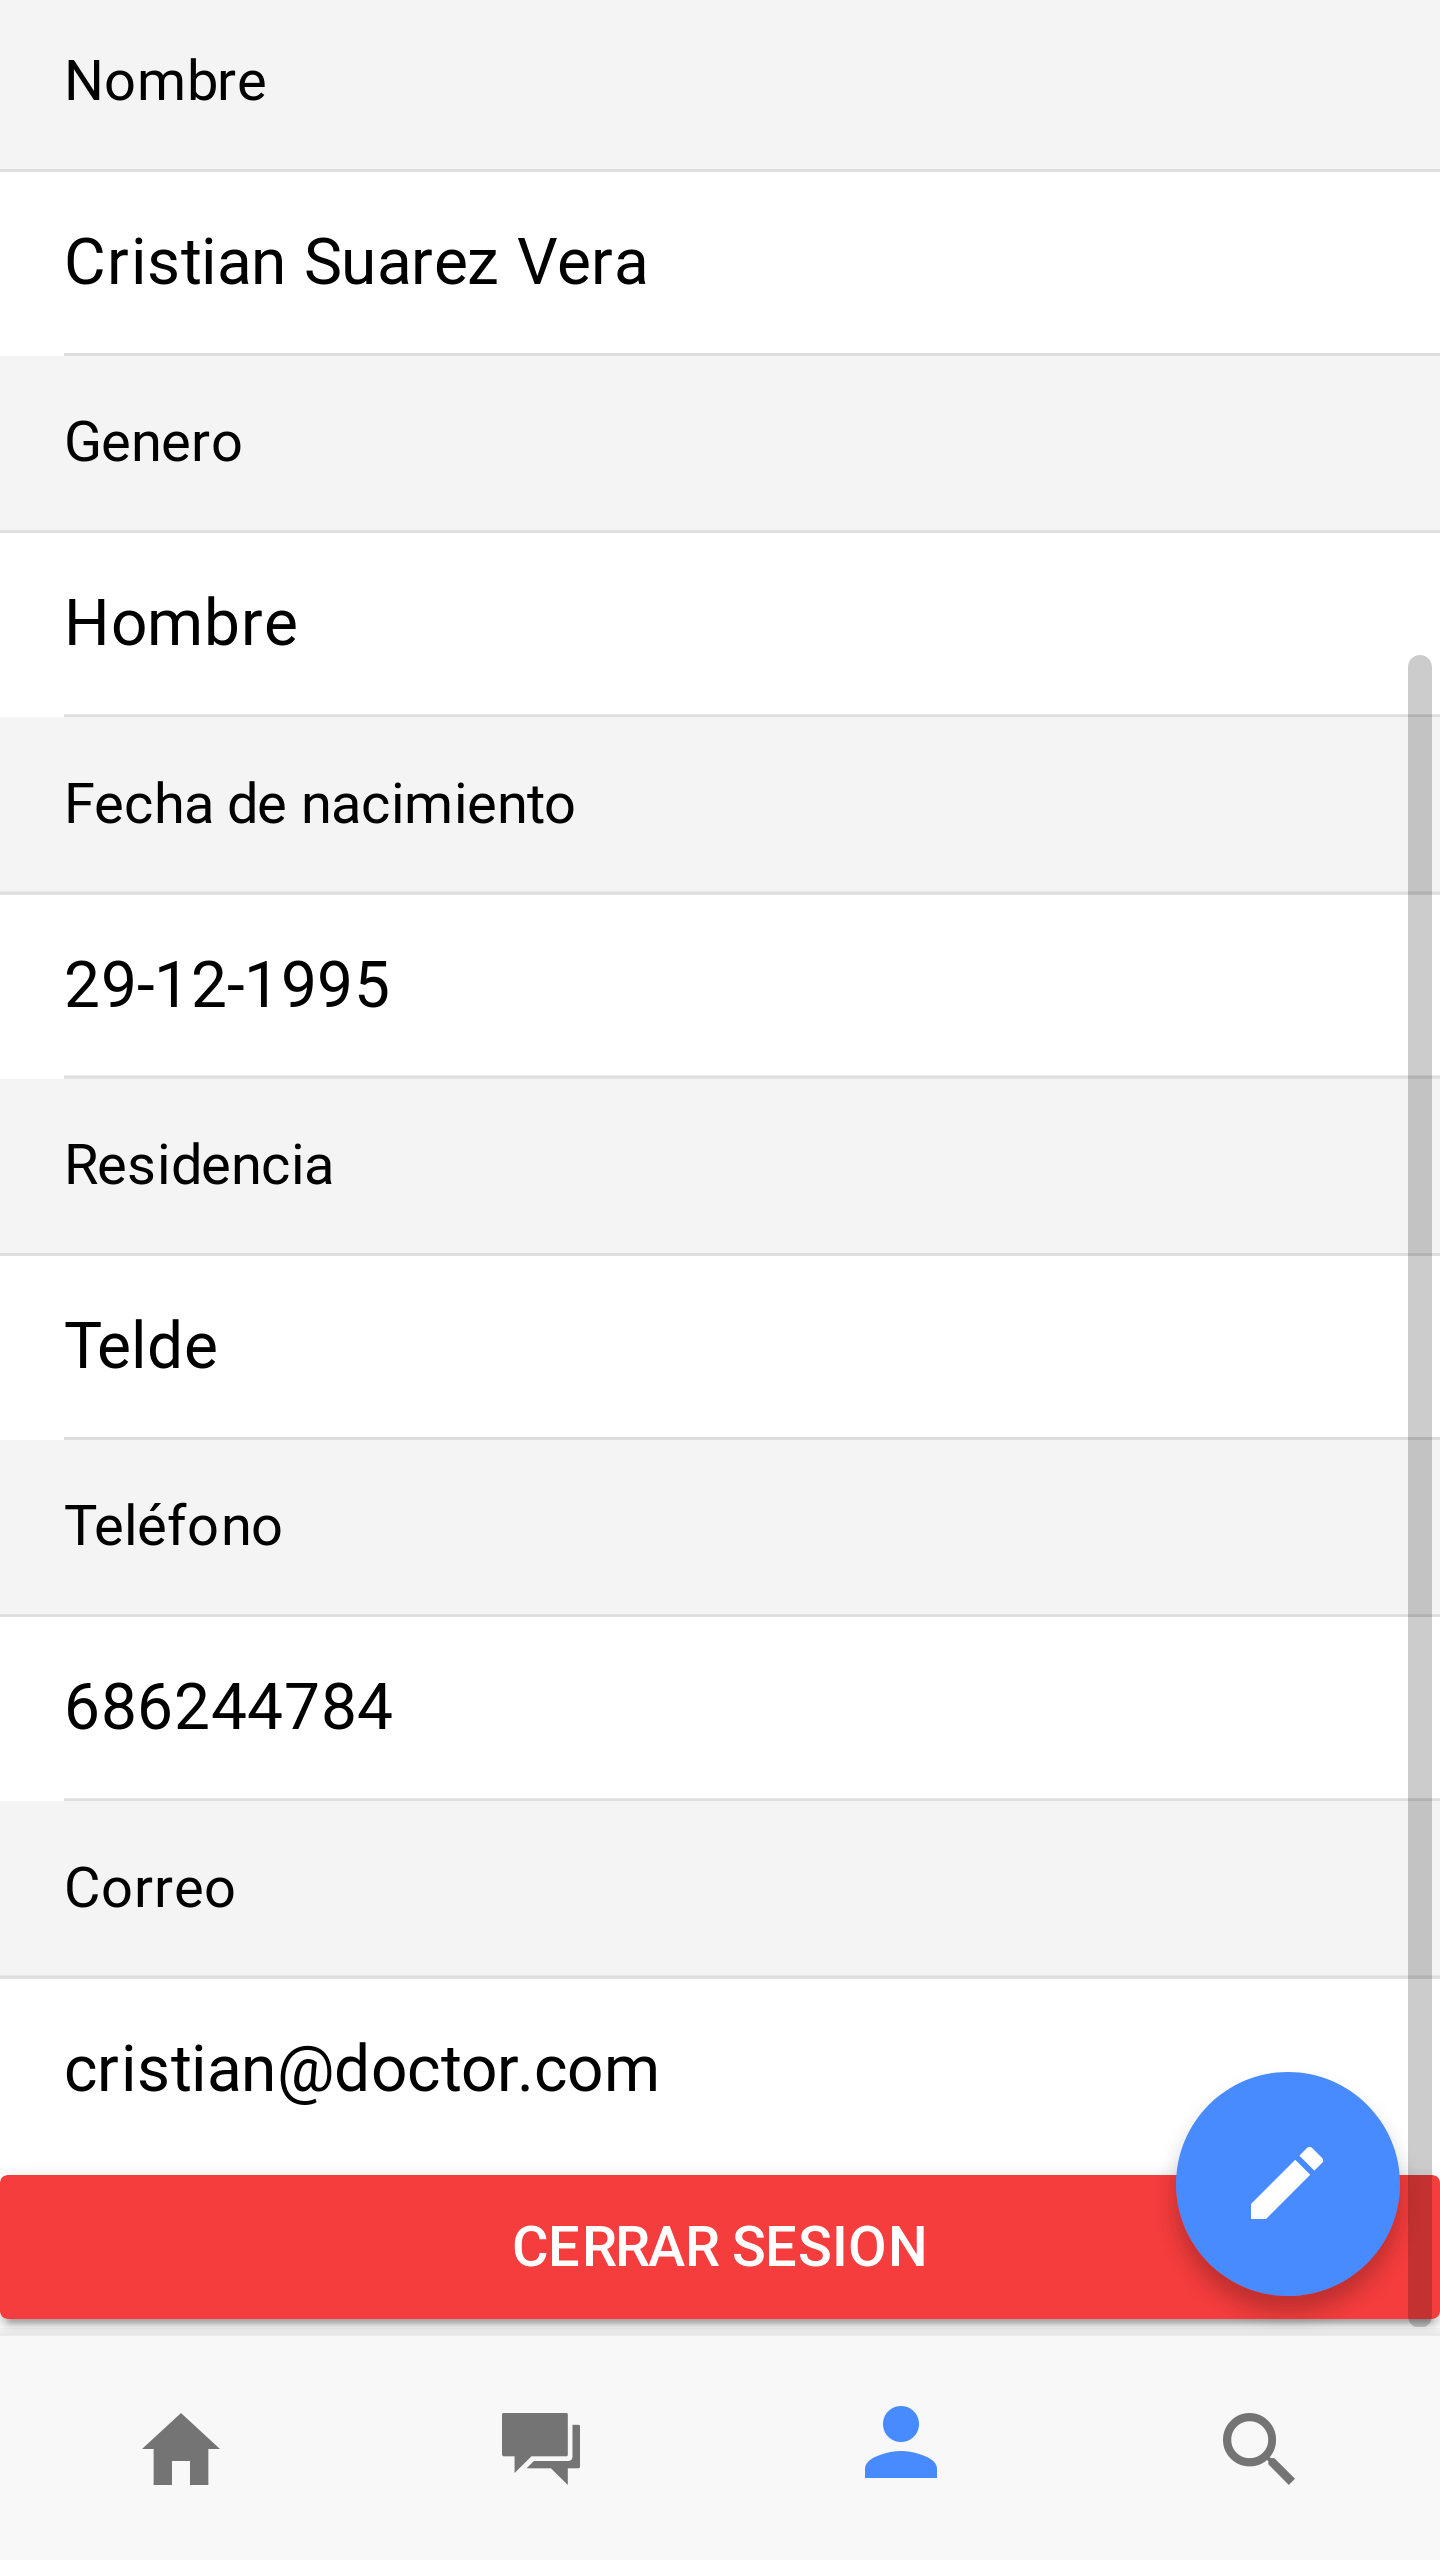
\includegraphics[width=0.5\textwidth]{images/screenshots/Perfil.png}
    \caption{Perfil de usuario}
    \label{perfil-usuario}
\end{figure}

Todos los usuarios tendrán disponible una vista como se muestra en la figura
\ref{perfil-usuario} en la que poder ver sus datos personales. Esta vista
además al final incluye un botón con el que pueden cerrar la sesión, si así
lo quisieran.
\clearpage

\subsection{Vista ejercicios, paciente}
\begin{figure}[!h]
    \centering
    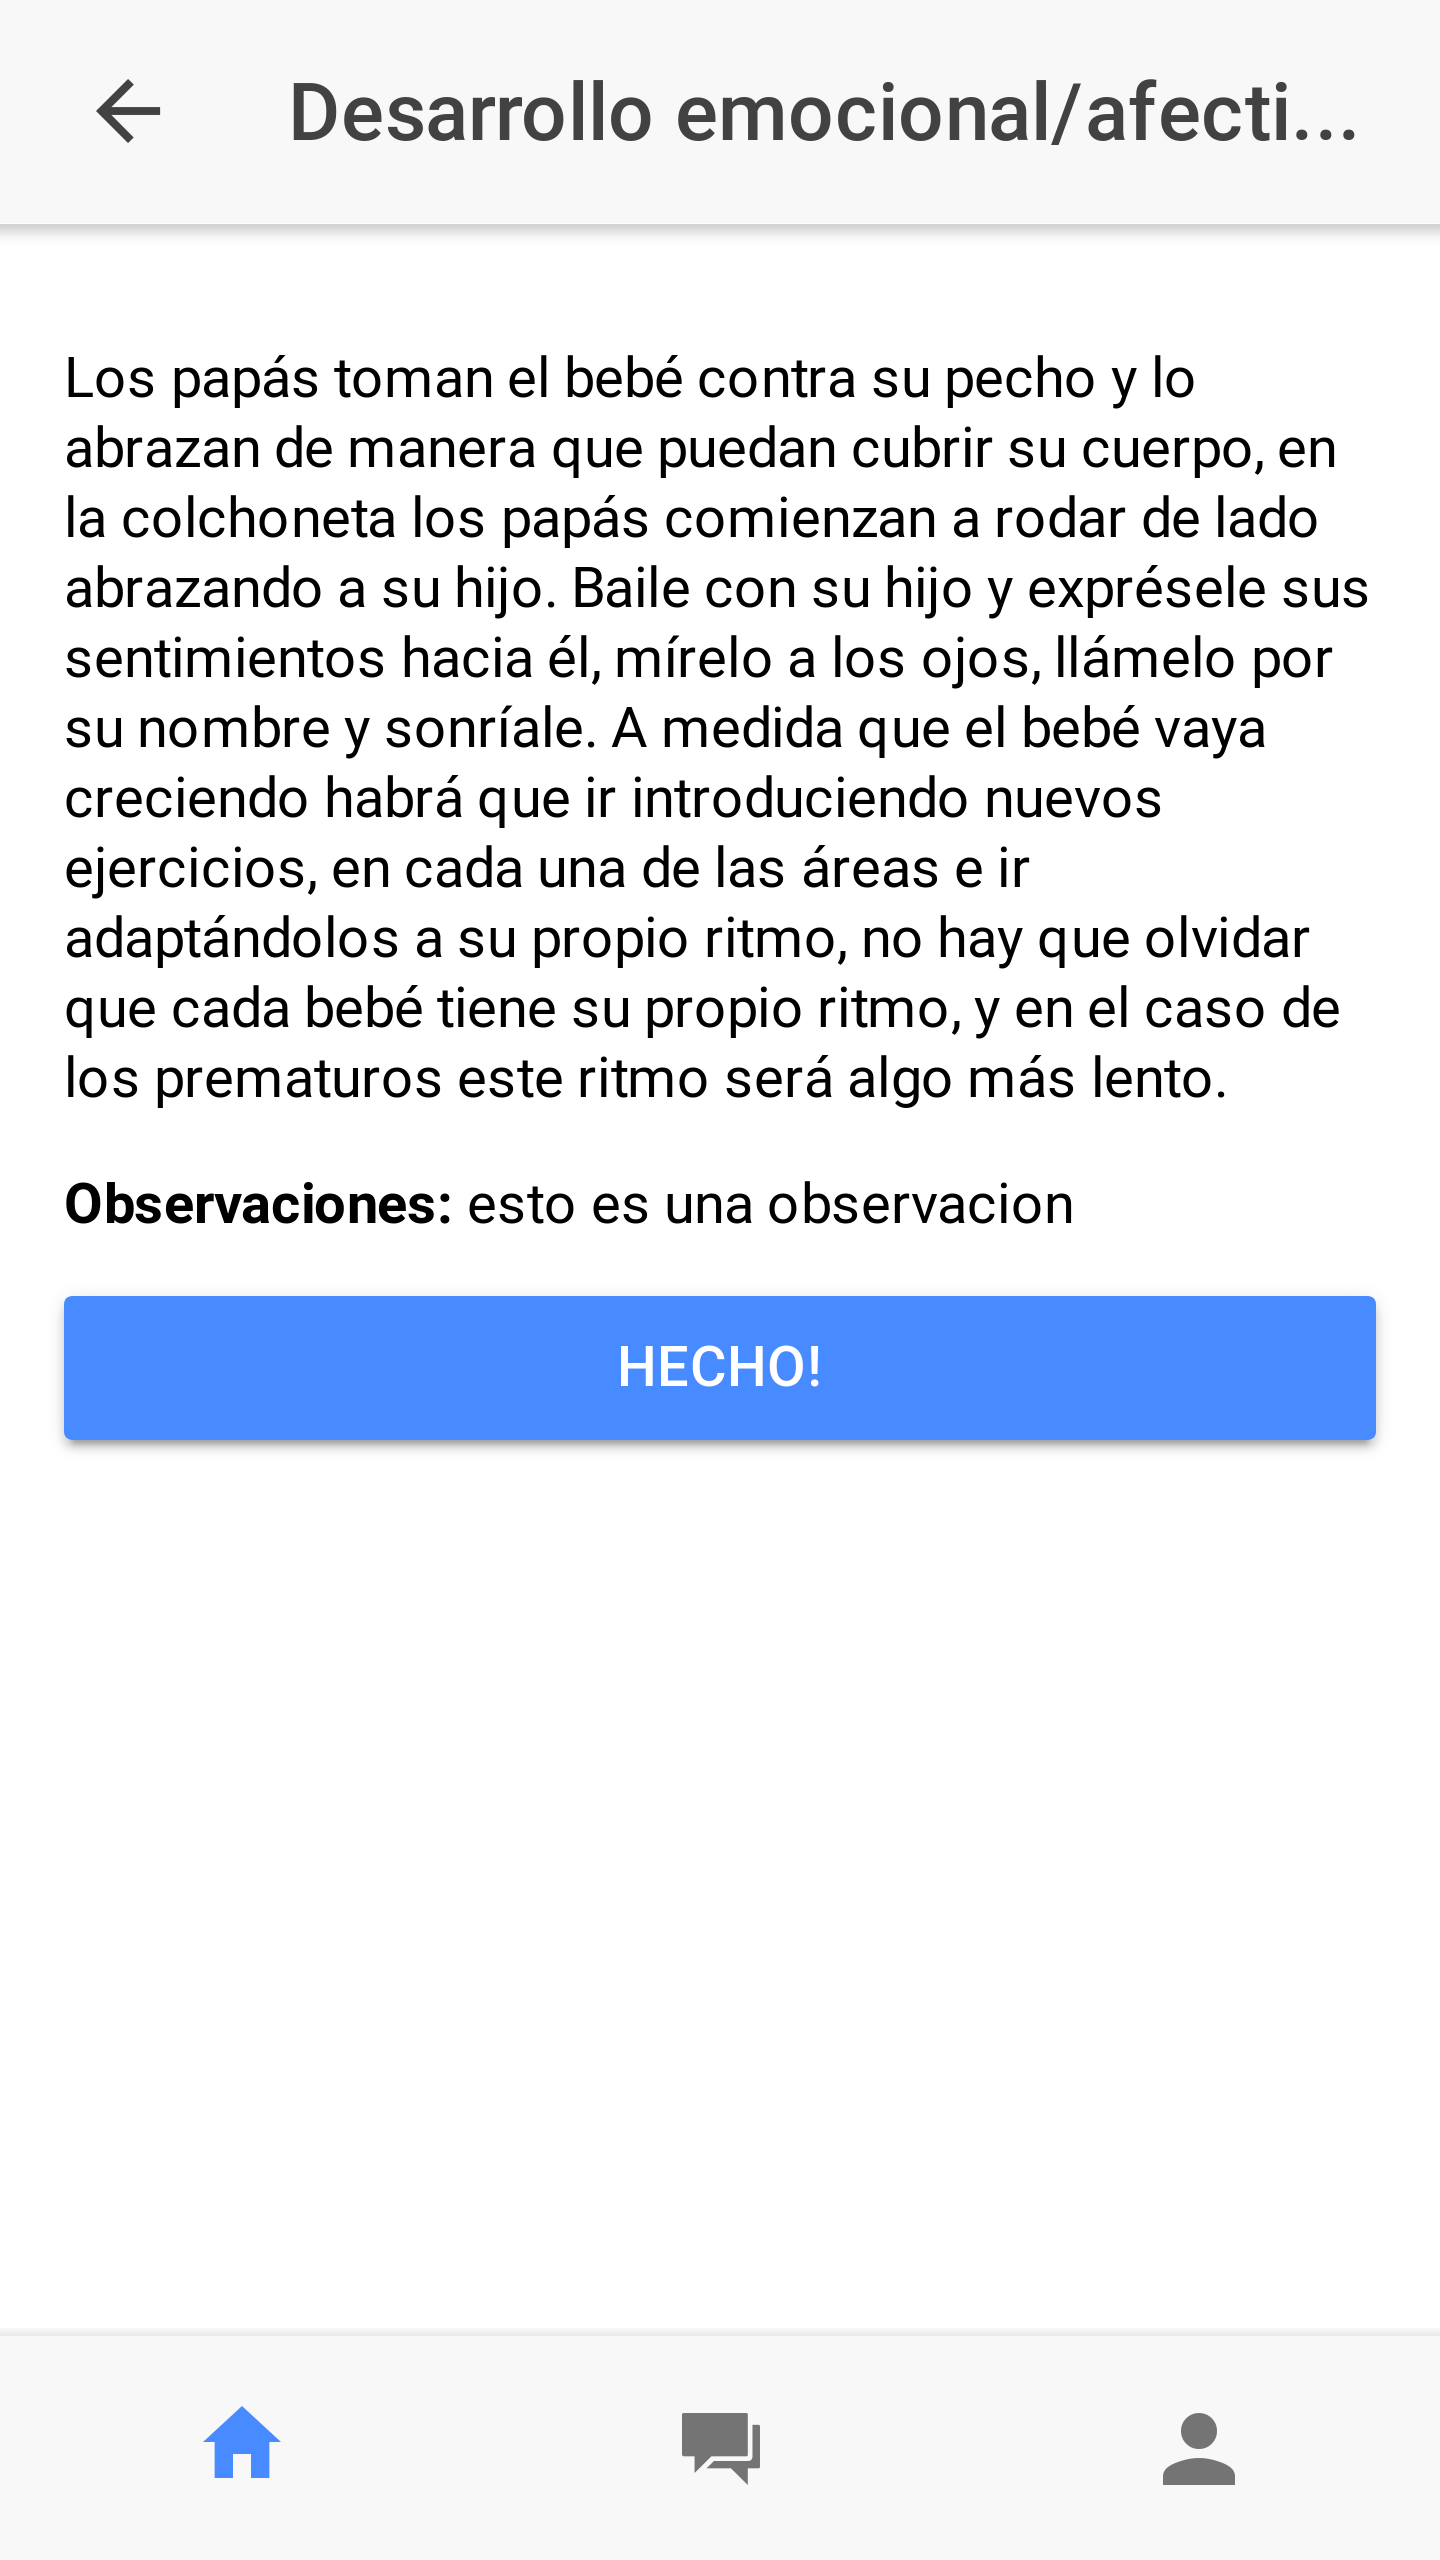
\includegraphics[width=0.5\textwidth]{images/screenshots/Paciente-vista-ejercicio-con-observaciones.png}
    \caption{Vista ejercicio con observaciones, paciente}
    \label{ejercicio-con-observaciones}
\end{figure}

Los pacientes al entrar a ver uno de los ejercicios que tiene asignados verá
la pantalla que se muestra en la figura \ref{ejercicio-con-observaciones}. En
esta podrá ver las especificaciones del ejercicio tales como la descripción y
las observaciones que el doctor puede haberle dejado indicadas. Además de
ello encontrará al final de esta un botón con el que podrá indicar si el
ejercicio ha sido completado.
\clearpage

\subsection{Vista ejercicios, doctor}
\begin{figure}[!h]
    \centering
    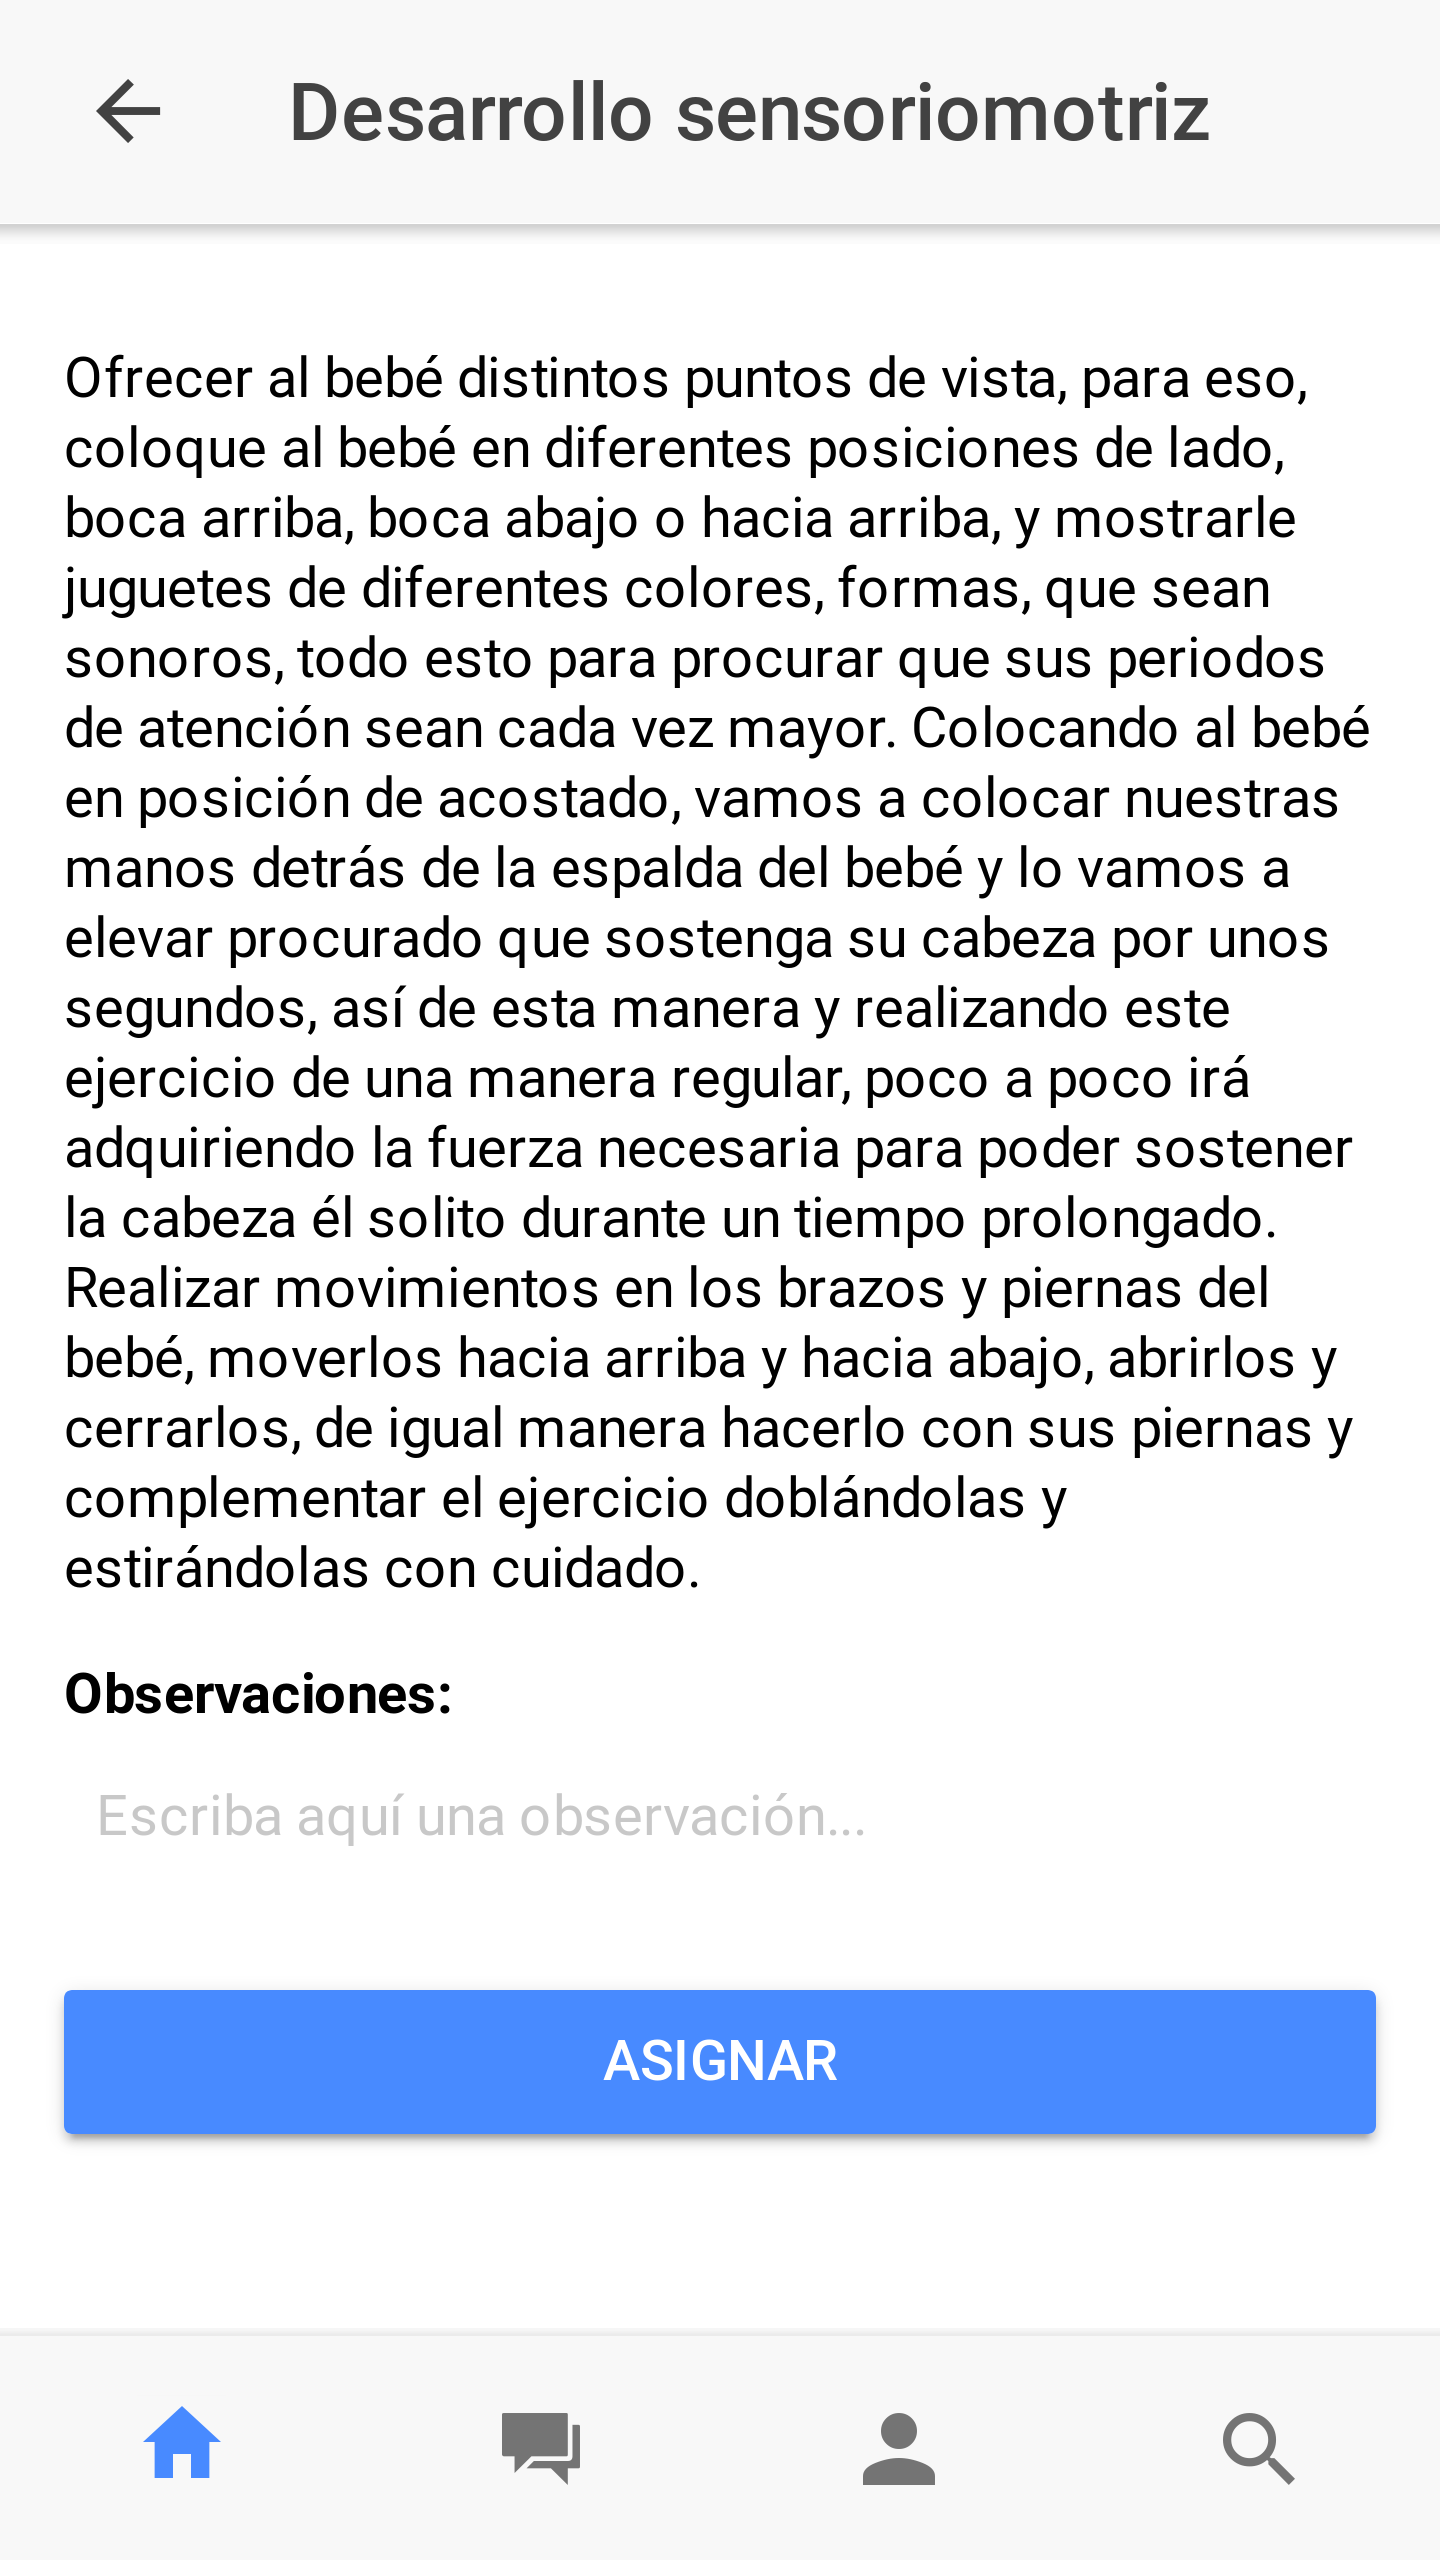
\includegraphics[width=0.5\textwidth]{images/screenshots/Doctor-anadir-observacion.png}
    \caption{Asignar ejercicio con observaciones, doctor}
    \label{asignar-ejercicio-con-observaciones}
\end{figure}

El doctor, una vez entra en la vista del ejercicio
(figura \ref{asignar-ejercicio-con-observaciones}) que quiere asignar a un
paciente tendrá a su dispocición un campo que puede completar o no con las
observaciones que quiera añadir. Para completar la asignación tendrá que
pulsar en el botón situado al final de la pantalla.
\clearpage

\subsection{Lista de chats}
\begin{figure}[!h]
    \centering
    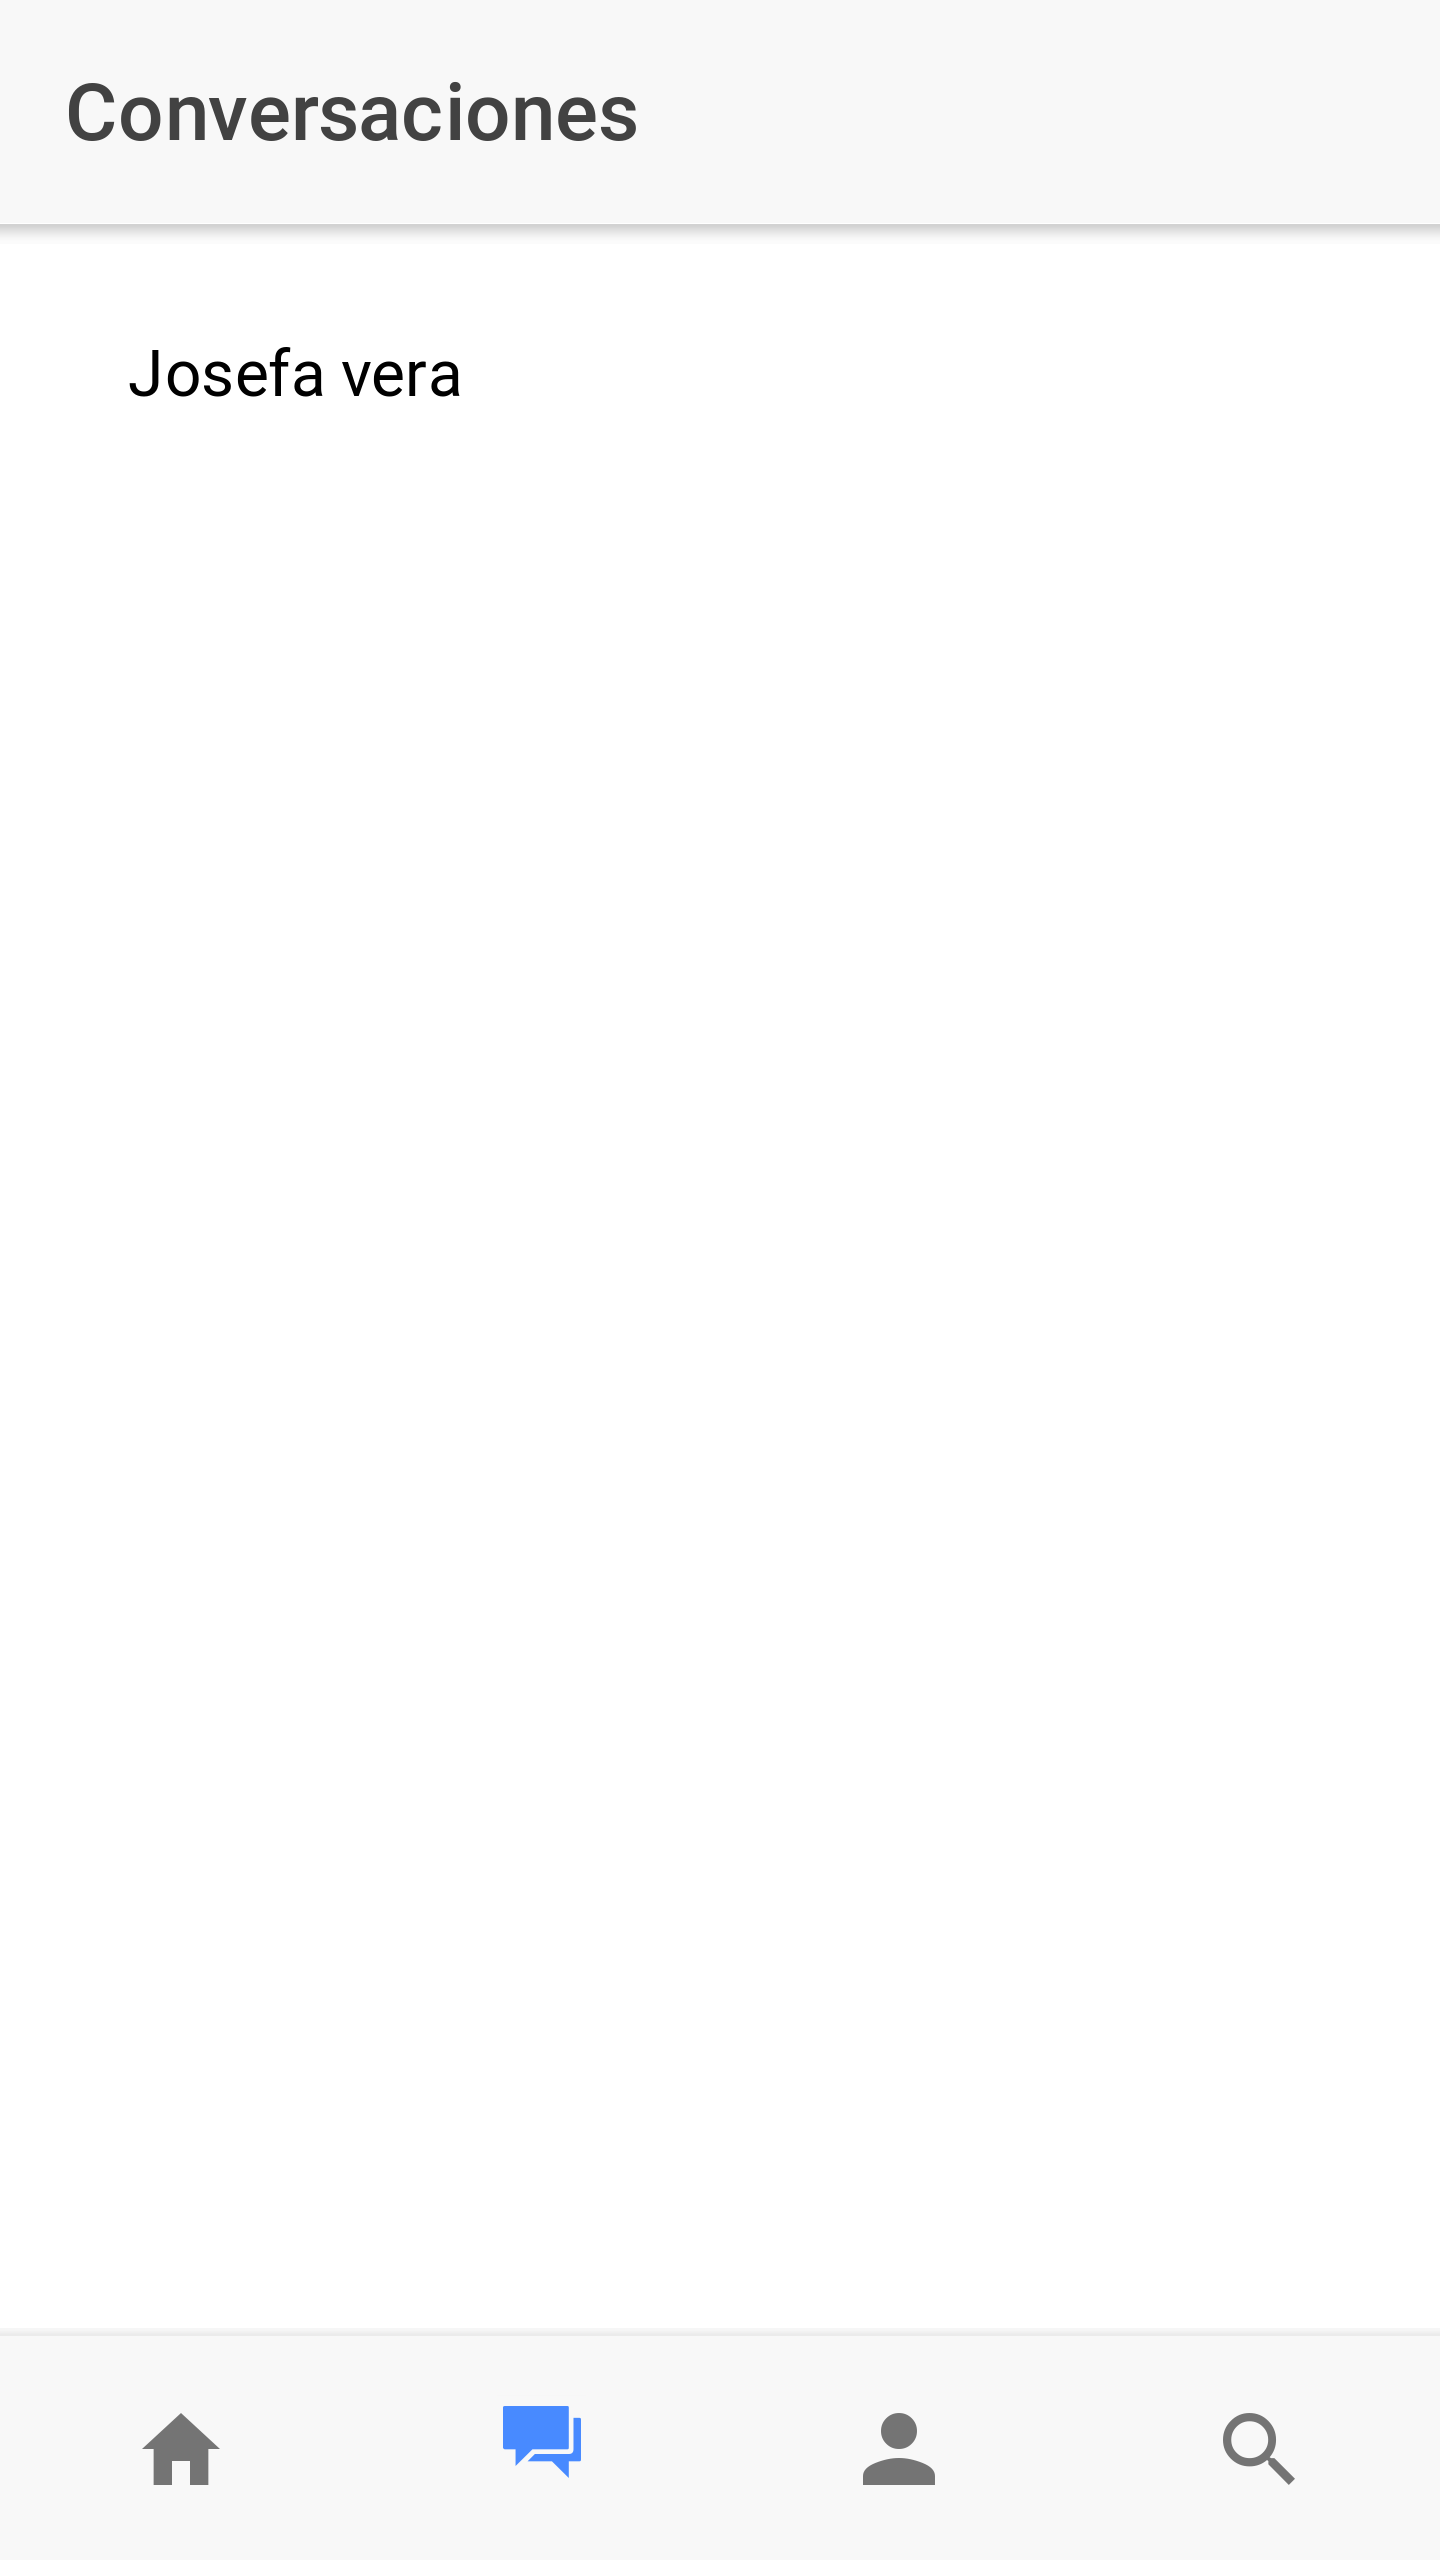
\includegraphics[width=0.5\textwidth]{images/screenshots/Doctor-vista-chats-abiertos.png}
    \caption{Chats abiertos}
    \label{vista-chats-abiertos}
\end{figure}

Todos los usuarios tendrán disponible una pantalla donde poder ver los chats
que tiene activos en ese momento, tal como se muestra en la figura
\ref{vista-chats-abiertos}.
\clearpage

\subsection{Mensajes de chat}
\begin{figure}[!h]
    \centering
    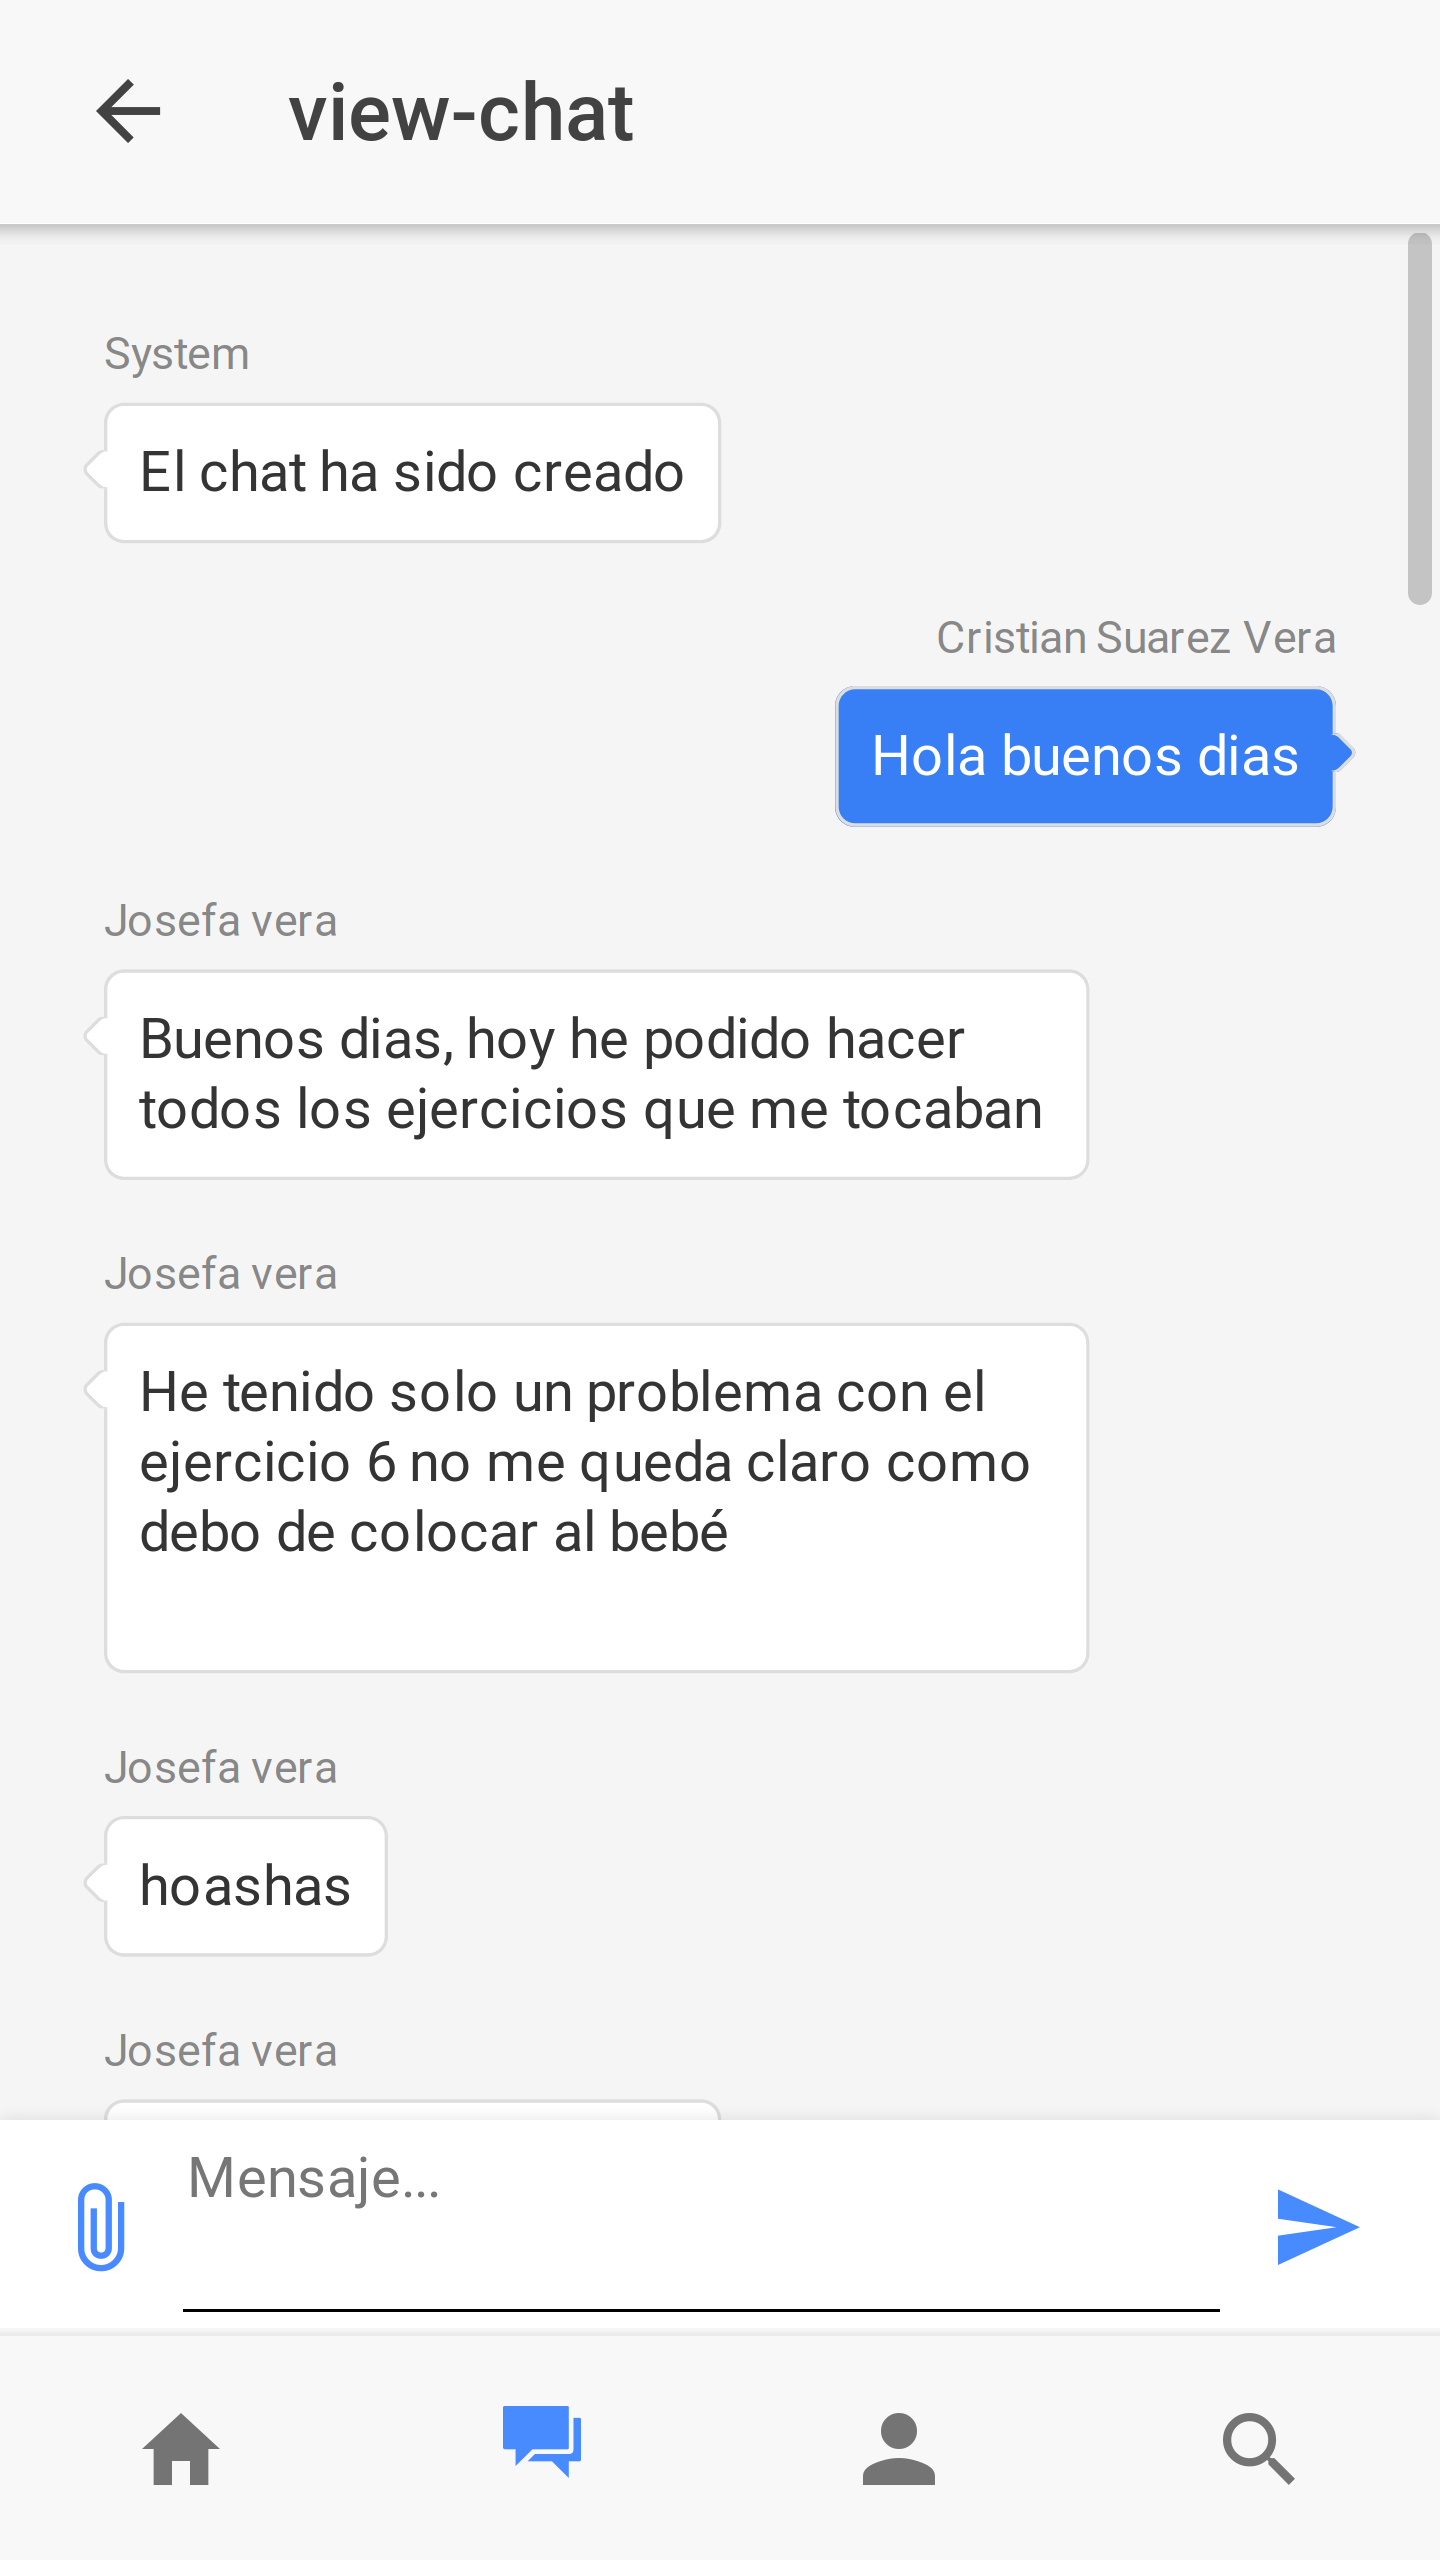
\includegraphics[width=0.5\textwidth]{images/screenshots/Vista-chat.png}
    \caption{Mensajes de un chat}
    \label{mensajes-chat}
\end{figure}

En la pantalla para el visionado de los mensajes del chat
(figura \ref{mensajes-chat}) los usuarios podrán ver la conversación que
mantiene con otro usuario. Además, se le permite enviar mensajes a este
completando el recuadro del final de la pantalla y pulsando sobre el botón
con forma de triángulo tumbado a la derecha.